\documentclass{book}
\usepackage[utf8]{inputenc}    
\usepackage{lmodern}
\usepackage[top=2.5cm, bottom=2.5cm, left=2.5cm, right=2.5cm]{geometry}
\usepackage{amsmath}
\usepackage{amsfonts}
\usepackage{amssymb}
\usepackage{amsthm}
\usepackage{calrsfs}
\usepackage{stmaryrd}
\usepackage{minted}
\usepackage{fancyhdr}
\usepackage[inline]{asymptote} 
\usepackage[linesnumbered,ruled,french,onelanguage]{algorithm2e}
\SetKwComment{Comment}{$\triangleright$\ }{}
\usepackage{hyperref}
\hypersetup{
    colorlinks,
    linktoc=section,
    linkcolor=red,
    urlcolor=orange,
    filecolor=red
}
\usepackage{times}
\usepackage{todonotes}
\usepackage{latexsym}
\usepackage{verbatim}
\usepackage{amsmath,amssymb}
\usepackage{upgreek}
\usepackage{dsfont}
\usepackage{framed}
\usepackage{amsfonts}
\newcommand{\tocheck}[1]{\textcolor{blue}{#1}}
\newcommand{\overbar}[1]{\mkern 3mu\overline{\mkern-3mu#1\mkern-3mu}\mkern 3mu}
\usepackage{fullpage,setspace}
\linespread{1.5}
\usepackage{enumerate}
\usepackage{mathrsfs}
\usepackage{amsthm}
\theoremstyle{definition}
\newtheorem{lemma}{Lemme}
\newtheorem{theorem}{Théorème}
\newtheorem{observation}[theorem]{Observation}
\newtheorem{definition}{Définition}
\newtheorem{heuristique}{Heuristique}
\newtheorem{scenario}{Scénario}
\newtheorem{fact}{Fait}
\newtheorem{example}{Exemple}
\newtheorem{postulate}{Postulat}
\newtheorem{proposition}{Proposition}
\newtheorem{corollary}{Corollaire}
\newtheorem{consequence}{Conséquence}
\newtheorem{property}{Propriété}
\numberwithin{lemma}{subsection}
\numberwithin{theorem}{subsection}
\numberwithin{definition}{subsection}
\numberwithin{proposition}{subsection}
\numberwithin{corollary}{subsection}
\numberwithin{property}{subsection}
\numberwithin{example}{subsection}
\numberwithin{heuristique}{subsection}
\numberwithin{scenario}{subsection}
\newenvironment{proofi} {\noindent\emph{Preuve~:}} {\hfill $\square$\vspace{0.2cm}}    

\title{Graphes et compléxité}
\author{
    Guillaume Pérution-Kihli\and
    Julien Rodriguez
}
\date{\today}

\begin{document}
\maketitle


\chapter{Introduction}

\begin{theorem}[Théoreme de Cook]
SAT est un problème NP-Complet. 
\end{theorem}

\begin{proposition}{2-SAT est un problème polynomial. Il appartient donc à la classe P.}
\end{proposition}

\begin{proofi}(Informelle)
Les différentes clauses $x \lor y$ peuvent être ré-écrites sous forme d'implications : $\neg x \rightarrow y$. À partir de ces implications, on construit un graphe d'implication (les variables deviennent des sommets reliés par un arc si une variable implique l'autre). On a la propriété suivante : si deux variables sont dans la même composante connexe, alors elles doivent avoir la même valeur. Et donc, si une variable et sa négation apparaissent dans la même composante connexe, alors la formule est insatisfiable. Si aucune composante connexe ne contient une variable et sa négation, alors la formule est satisfiable. On peut calculer les composantes fortement connexes à l'aide d'un algorithme polynomial comme celui de Tarjan. Par conséquent, et puisque notre réduction est polynomial, le problème 2-SAT peut se résoudre en temps polynomial.

\end{proofi}


\begin{proposition} Tous les problèmes NP-Complets sont équivalents du point de vue de la réduction polynomiale.
\end{proposition}

\begin{proofi}
Par définition d'un problème NP-complet A, tous les problèmes de la classe NP se réduisent à A par une réduction polynomiale. Donc tout problème NP-complet B se réduit à A et inversement : ces problèmes sont équivalents du point de vue de la réduction polynomiale.
\end{proofi}

\begin{consequence}
Les problèmes NP-complet sont tous aussi difficiles les uns que les autres.
\end{consequence}

\section{Vertex Cover}

\begin{definition}[Vertex Cover]
Soient un graphe $G = (V, E)$, avec $V$ un ensemble de sommets et $E$ un ensemble d'arêtes et un entier $k \in \mathbb{N}$. \\
$VC(G, k) = \mbox{existe-t-il } S \subseteq V $ avec $ \left | S \right | \leqslant k \mbox{ tel que } \forall (u, v) \in E^2,~u \in S$ ou $v \in S$ ? 
\end{definition}

\begin{example}
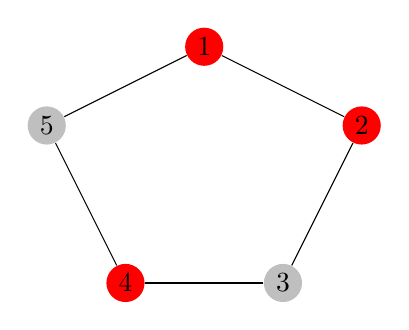
\begin{tikzpicture}[shorten >=1pt,->]
  \tikzstyle{vertex}=[circle,fill=black!25,minimum size=12pt,inner sep=2pt]
  \node[vertex, fill=red] (G_1) at (0,2) {1};
  \node[vertex, fill=red] (G_2) at (2,1)   {2};
  \node[vertex] (G_3) at (1,-1) {3};
  \node[vertex, fill=red] (G_4) at (-1,-1)   {4};
  \node[vertex] (G_5) at (-2,1) {5};
  
  \draw (G_1) -- (G_2) -- cycle;
  \draw (G_2) -- (G_3) -- cycle;
  \draw (G_3) -- (G_4) -- cycle;
  \draw (G_4) -- (G_5) -- cycle;
  \draw (G_5) -- (G_1) -- cycle;
\end{tikzpicture}
\end{example}

\begin{algorithm}[H]\label{algo:vertexCover}
\caption{Vertex Cover (Algorithme de branchement)} 
\SetAlgoLined
\DontPrintSemicolon
\SetAlgoLined
\DontPrintSemicolon
\SetKwInOut{Input}{entrées}
\SetKwInOut{Output}{sortie}
\SetKwInOut{Variables}{Variables}
\Input{un graphe $G = (V, E)$, un entier $k \in \mathbb{N}$}
\Output{un ensemble $S \subseteq V$}
    
    \While{\textit{il existe un arête} $(x, y) \in E \mbox{ et } k \geqslant 1$}
    {
        $VC(G-x, k-1)$\;
        $VC(G-y, k-1)$\;
    }
    \Return $k == 1$
\end{algorithm}

Complexité en $O(2^k*n^{O(1)})$.

Vertex Cover $\in FPT \Leftrightarrow f(k)*n^{O(1)}$.

\section{Independant Set (stable)}

\begin{definition}[Independant Set]
Soient un graphe $G = (V, E)$ et un entier $k \in \mathbb{N}$. \\
$IS(G, k) = \mbox{ existe-t-il } S \subseteq V $ avec $ \left | S \right | \geqslant k \mbox{ tel que } \forall (u, v) \in S^2, \{u, v\} \notin E$ ?
\end{definition}

Pour résoudre le problème de l'ensemble indépendant, on peut réutiliser l'algorithme du Vertex-Cover (algo. \ref{algo:vertexCover}) car il s'agit du complémentaire de ce problème. Ce qui donnerait une complexité en $O(2^{n-k}*n^{O(1)}$.
Il est aussi possible d'utiliser une variante où l'on teste tous les sous-ensembles de $V$ de taille $k$ et dans ce cas, la complexité est de $O(n^k)$.

Conjecture : mieux ? non. 

Independant Set $\in XP \Leftrightarrow n^{f(k)}$.

\section{Coloration}

\begin{definition}[Coloration]
Soient un graphe $G = (V, E)$ et un entier $k \in \mathbb{N}$. Soit $\mathcal{P}$ une partition de $V$ en ensembles indépendants. \\
$COL(G, k) = \mbox{ existe-t-il } \mathcal{P} \mbox{ tel que } \left | \mathcal{P} \right | \leqslant k$ ?
\end{definition}

Coloration $\in para NP-Complet$, pour un $k$ fixé, le problème de la coloration appartient à la classe $NP-Complet$.

\chapter{Graphes triangulés}

Autres noms : graphes chordaux, graphes de Gallai.

\begin{proposition}
On limite la taille des cycles.
\end{proposition}

\section{Définitions}

\begin{definition}
Soient un graphe $G=(V, E)$. $G$ est triangulé, si tout cycle de G de longueur (nombre de sommets) au moins 4 possède une corde.
\end{definition}

\begin{definition}
Une arête entre 2 sommets non-consécutifs d'un cycle est une corde.
\end{definition}

\begin{example}
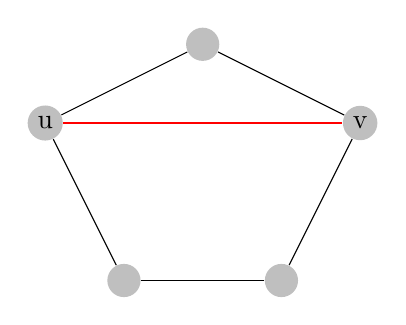
\begin{tikzpicture}[shorten >=1pt,->]
  \tikzstyle{vertex}=[circle,fill=black!25,minimum size=12pt,inner sep=2pt]
  \node[vertex] (G_1) at (0,2) {};
  \node[vertex] (G_2) at (2,1)   {v};
  \node[vertex] (G_3) at (1,-1) {};
  \node[vertex] (G_4) at (-1,-1)   {};
  \node[vertex] (G_5) at (-2,1) {u};
  
  \draw (G_1) -- (G_2) -- cycle;
  \draw (G_2) -- (G_3) -- cycle;
  \draw (G_3) -- (G_4) -- cycle;
  \draw (G_4) -- (G_5) -- cycle;
  \draw (G_5) -- (G_1) -- cycle;
  \draw[red] (G_5) -- (G_2) -- cycle;
\end{tikzpicture}

L'arête $(u, v)$ est une corde.
\end{example}

\begin{example}
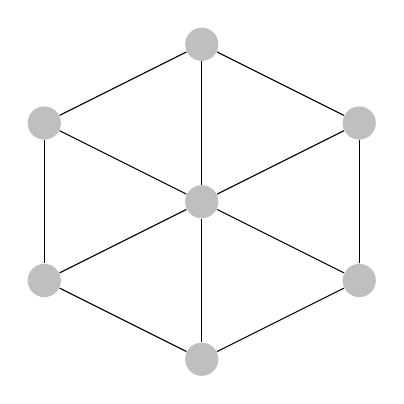
\begin{tikzpicture}[shorten >=1pt,->]
  \tikzstyle{vertex}=[circle,fill=black!25,minimum size=12pt,inner sep=2pt]
  \node[vertex] (G_0) at (0,0) {};
  \node[vertex] (G_1) at (0,2) {};
  \node[vertex] (G_2) at (2,1)   {};
  \node[vertex] (G_3) at (2,-1) {};
  \node[vertex] (G_4) at (0,-2)   {};
  \node[vertex] (G_5) at (-2,-1) {};
  \node[vertex] (G_6) at (-2,1) {};
  
  \draw (G_1) -- (G_2) -- cycle;
  \draw (G_2) -- (G_3) -- cycle;
  \draw (G_3) -- (G_4) -- cycle;
  \draw (G_4) -- (G_5) -- cycle;
  \draw (G_5) -- (G_6) -- cycle;
  \draw (G_6) -- (G_1) -- cycle;
  \draw (G_1) -- (G_0) -- cycle;
  \draw (G_2) -- (G_0) -- cycle;
  \draw (G_3) -- (G_0) -- cycle;
  \draw (G_4) -- (G_0) -- cycle;
  \draw (G_5) -- (G_0) -- cycle;
  \draw (G_6) -- (G_0) -- cycle;
\end{tikzpicture}

$G$ est-il triangulé ? NON!
\end{example}

\begin{example}
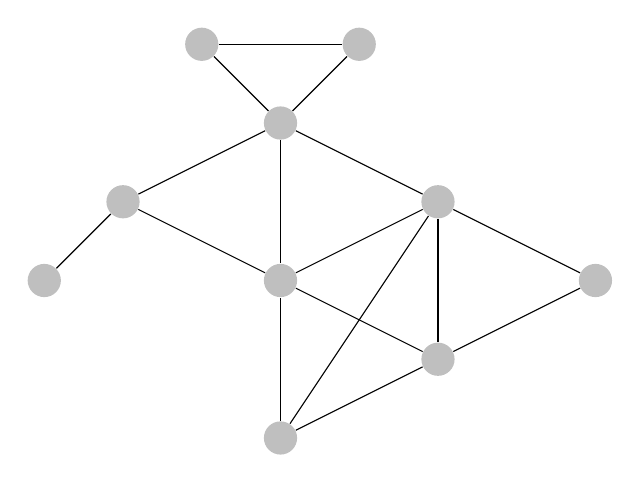
\begin{tikzpicture}[shorten >=1pt,->]
  \tikzstyle{vertex}=[circle,fill=black!25,minimum size=12pt,inner sep=2pt]
  \node[vertex] (G_0) at (0,0) {};
  \node[vertex] (G_1) at (0,2) {};
  \node[vertex] (G_2) at (2,1)   {};
  \node[vertex] (G_3) at (2,-1) {};
  \node[vertex] (G_4) at (0,-2)   {};
  \node[vertex] (G_6) at (-2,1) {};
  
  \node[vertex] (G_7) at (4,0)   {};
  
  \node[vertex] (G_8) at (-1,3)   {};
  \node[vertex] (G_9) at (1,3)   {};
  
  \node[vertex] (G_10) at (-3,0)   {};
  
  \draw (G_1) -- (G_2) -- cycle;
  \draw (G_2) -- (G_3) -- cycle;
  \draw (G_3) -- (G_4) -- cycle;
  \draw (G_2) -- (G_4) -- cycle;
  \draw (G_6) -- (G_1) -- cycle;
  \draw (G_1) -- (G_0) -- cycle;
  \draw (G_2) -- (G_0) -- cycle;
  \draw (G_3) -- (G_0) -- cycle;
  \draw (G_4) -- (G_0) -- cycle;
  \draw (G_6) -- (G_0) -- cycle;
  
  \draw (G_2) -- (G_7) -- cycle;
  \draw (G_3) -- (G_7) -- cycle;
  
  \draw (G_1) -- (G_8) -- cycle;
  \draw (G_1) -- (G_9) -- cycle;
  \draw (G_8) -- (G_9) -- cycle;
  
  \draw (G_6) -- (G_10) -- cycle;
  
\end{tikzpicture}

$G$ est triangulé.
\end{example}


\begin{example}
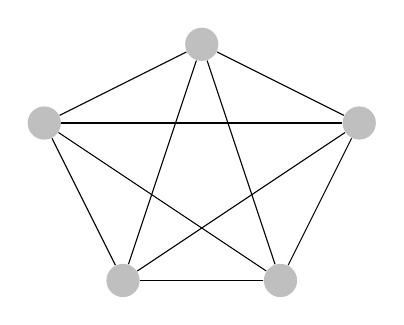
\begin{tikzpicture}[shorten >=1pt,->]
  \tikzstyle{vertex}=[circle,fill=black!25,minimum size=12pt,inner sep=2pt]
  \node[vertex] (G_1) at (0,2) {};
  \node[vertex] (G_2) at (2,1)   {};
  \node[vertex] (G_3) at (1,-1) {};
  \node[vertex] (G_4) at (-1,-1)   {};
  \node[vertex] (G_5) at (-2,1) {};
  
  \draw (G_1) -- (G_2) -- cycle;
  \draw (G_1) -- (G_3) -- cycle;
  \draw (G_1) -- (G_4) -- cycle;
  \draw (G_1) -- (G_5) -- cycle;
  
  \draw (G_2) -- (G_3) -- cycle;
  \draw (G_2) -- (G_4) -- cycle;
  \draw (G_2) -- (G_5) -- cycle;
  
  \draw (G_3) -- (G_4) -- cycle;
  \draw (G_3) -- (G_5) -- cycle;
  
  \draw (G_4) -- (G_5) -- cycle;
 
\end{tikzpicture}

$\forall n \in \mathbb{N}, K_n$ est triangulé.
\end{example}

Les graphes acycliques (forêt) sont triangulés.

\subsection{Séparateurs et ordres d'éliminations}

\begin{definition}
Soient $G = (V, E)$ un graphe et $S \leqslant V$. $S$ est un séparateur si $G-S = G[V\\S]$ contient plus de composantes connexes que $G$.
\end{definition}

\begin{example}
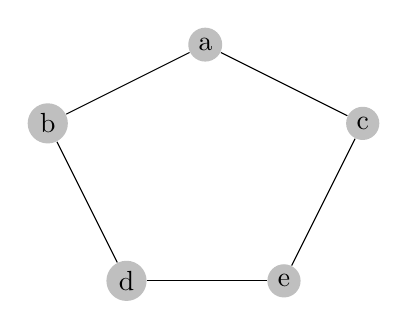
\begin{tikzpicture}[shorten >=1pt,->]
  \tikzstyle{vertex}=[circle,fill=black!25,minimum size=12pt,inner sep=2pt]
  \node[vertex] (G_1) at (0,2) {a};
  \node[vertex] (G_2) at (2,1)   {c};
  \node[vertex] (G_3) at (1,-1) {e};
  \node[vertex] (G_4) at (-1,-1)   {d};
  \node[vertex] (G_5) at (-2,1) {b};
  
  \draw (G_1) -- (G_2) -- cycle;
  \draw (G_1) -- (G_5) -- cycle;
 
  
  \draw (G_2) -- (G_3) -- cycle;
  
  
  \draw (G_3) -- (G_4) -- cycle;
  
  \draw (G_4) -- (G_5) -- cycle;
 
\end{tikzpicture}

$\{b, c, e \}$ est séparateur. $\{b, c\}$ est aussi un séparateur.
\end{example}

\begin{definition}
$s$ est un (ab)-séparateur de $G$ si $a$ et $b$ sont connectés dans $G$ mais pas dans $G-s$.
\end{definition}

\begin{example}
$\{b, c, e\}$ est un (ad)-séparateur et $\{ b, c\}$ est un (ad)-séparateur minimal.
\end{example}

\begin{definition}
$s$ est un (ab)-séparateur minimal, si $s$ est un (ab)-séparateur et $\forall s' \subseteq  $, $s'$ n'est pas un (ab)-séparateur.
\end{definition}

\begin{definition}
$s$ est un (ab)-séparateur minimal, si $\exists a, b \in V$, $s$ est un (ab)-séparateur minimal. 
\end{definition}

\begin{example}
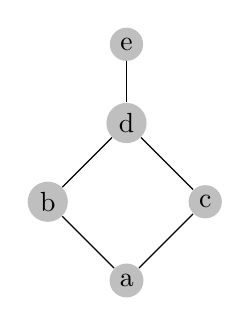
\begin{tikzpicture}[shorten >=1pt,->]
  \tikzstyle{vertex}=[circle,fill=black!25,minimum size=12pt,inner sep=2pt]
  \node[vertex] (G_1) at (0,2) {e};
  \node[vertex] (G_2) at (0,1)   {d};

  \node[vertex] (G_4) at (-1,0)   {b};
  \node[vertex] (G_5) at (1,0) {c};
   \node[vertex] (G_6) at (0,-1) {a};
  
  \draw (G_1) -- (G_2) -- cycle;
  \draw (G_2) -- (G_4) -- cycle;
 \draw (G_2) -- (G_5) -- cycle;
 \draw (G_6) -- (G_4) -- cycle;
 \draw (G_6) -- (G_5) -- cycle;
\end{tikzpicture}

$(a, d)$ est-il un séparateur minimal ? oui (pas pour les mêmes paires). Mais aussi $\{d\}$ est un séparateur-min.
\end{example}

\begin{definition}
Un ordre d'élimination d'un graphe $G$ est une permutation de ses sommets : $\sigma = x_1 ... x_i ... x_n$

$G_i = [V_i]$ avec $V_i = \{x_i,...,x_n\}$, $\sigma$ est un $\pi$-ordre d'élimination si $\forall i \in [n]$, $x_i$ vérifie la propriétée $\pi$ dans $G_i$
\end{definition}

\begin{example}
Les forêts admettent un ordre d'élimination par feuille.
\end{example}

\section{Les forêts}

\begin{theorem}
Soit $G = (V, E)$ un graphe, les propositions suivantes sont équivalentes :
\begin{enumerate}
    \item $G$ est acyclique
    \item $G$ possède un ordre d'élimination par feuille
    \item Tout séparateur minimal de $G$ est un singleton et $K_3 \nsubseteq G$ 
\end{enumerate}
\end{theorem}


\begin{proofi}
\begin{itemize}
    \item (1 $\implies$ 3). $G$ acyclique $\implies K_3 \nsubseteq G \implies$ il existe un seul chemin des feuilles. Si $G$ contient $K_t$, avec $t \geqslant 3$ alors $G$ contient un cycle. Supposons que $G$ possède un séparateur minimal $S$ de taille au moins 2.
    %schema
    Puisque $S$ est minimal il existe 2 composantes connexes $A$ et $B$ tel que $\forall x \in S$, $N(x) \cap A \neq  \emptyset$ et $N(x) \cap B \neq  \emptyset$. 
    
    Soient $u$, $v \in S$ alors $\exists u_A, v_A \in A, u_B, v_B \in B$ tel que $\{(u_A, u), (u_B, u), (v_A, v), (v_B, v)\} \in E $ et il existe un chemin dans $A$ entre $u_A$ et $v_A$, $P_A$ et un chemin dans $B$ entre $u_B$ et $v_B$, $P_B$. On a donc que $uu_AP_Av_Avv_BP_Bu_Bu$ est un cycle.
    \item (3 $\implies$ 2). Soit $s$ un séparateur minimal extrême, $G-s$ contient une composante connexe $C$ telle que $G[S \cup C]$ ne contient pas de séparateur (clique). $G[S \cup C]$ est un $K_2$ donc une arête. $C$ est réduite à un sommet de degré 1 : une feuille.
    Hypothèse : $|C| \geqslant 2$. Supposons que $N(x) \cap C$ = $\{ y \} \implies \{ y \}$ est un séparateur min. Contradiction. Donc $x$ possède au moins 2 voisins $x$ et $y$ reliés par un chemin $P$ dans $C \implies xyPy\prime x$ est un cycle non complet.
    %schema
    \item (2 $\implies$ 1). Ajouter une feuille ne créer pas de cycle donc si $G$ possède un ordre d'élimination par feuille $G$ est acyclique.
\end{itemize}
\end{proofi}
  
\begin{theorem}
  \begin{enumerate}
        \item $G$ est triangulé
        \item $G$ possède un ordre d'élimination simplicial
        \item Tout séparateur minimal de $G$ est complet
    \end{enumerate}
\end{theorem}

\begin{example}
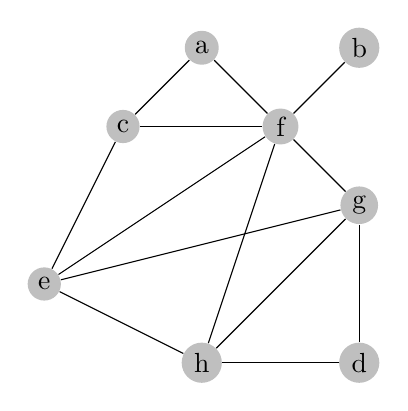
\begin{tikzpicture}[shorten >=1pt,->]
  \tikzstyle{vertex}=[circle,fill=black!25,minimum size=12pt,inner sep=2pt]
  \node[vertex] (G_0) at (-1,0) {e};
  \node[vertex] (G_1) at (0,2) {c};
  \node[vertex] (G_5) at (1,3) {a};
  \node[vertex] (G_2) at (2,2)   {f};
  \node[vertex] (G_3) at (3,1) {g};
  \node[vertex] (G_4) at (1,-1)   {h};
   \node[vertex] (G_6) at (3,3)   {b};
    \node[vertex] (G_7) at (3,-1) {d};
    
\draw (G_7) -- (G_3) -- cycle;
  \draw (G_7) -- (G_4) -- cycle;


  \draw (G_6) -- (G_2) -- cycle;
  
  \draw (G_5) -- (G_2) -- cycle;
  \draw (G_5) -- (G_1) -- cycle;

  
  \draw (G_1) -- (G_2) -- cycle;
  \draw (G_2) -- (G_3) -- cycle;
  \draw (G_3) -- (G_4) -- cycle;
  \draw (G_2) -- (G_4) -- cycle;

  \draw (G_1) -- (G_0) -- cycle;
  \draw (G_2) -- (G_0) -- cycle;
  \draw (G_3) -- (G_0) -- cycle;
  \draw (G_4) -- (G_0) -- cycle;

 
  

  
\end{tikzpicture}
\newline
$abcdefgh$ est un ordre d'élimination simplicial.
\end{example}

\begin{proofi}
\begin{itemize}
    \item ( $1 \implies 3$ ). Hypothèse : $\exists s$, un séparateur-min contenant 2 sommets $a$ et $b$ non adjacent. %schema 
    Alors, il existe un chemin $P_A$ entre $x$ et $y$ tels que tous les sommets internes sont dans $A$, il existe un chemin $P_B$ entre $x$ et $y$ tels que tout les sommets internes sont dans $B$.
    On choisit $P_A$ et $P_B$ de longueur minimum. $P_AP_B$ forme un cycle sans corde de ongueur supérieur ou égale à 4. Contradiction.
    \item ( $3 \implies 2$ ). Hypothèse : $G$ n'est pas complet, alors il existe un séparateur minimal $s$. Si $G_A$ est complet alors il existe un sommet $x_A \in A$ qui est simplicial. Si $G_A$ n'est pas complet il existe 2 sommets simpliciaux non adjacent alors l'un des deux est $A$ car $S$ est complet, alors il existe $x_A \in A, x_B \in B$ simpliciaux et $x_Ax_B \notin E$.
    \item ( $2 \implies 1$ ).
\end{itemize}
\end{proofi}

\section{Modèle d'intersection et arbre de cliques}

\begin{definition}{Graphes d'intersection}
Soit $\mathcal{F} = \{S_1, ... , S_n \}$ une famille d'ensemble de "trucs". Soit $G = (V, E)$ est le graphe d'intersection de $\mathcal{F}$ si $V = \{ x_1, ..., x_n\}$ et $x_ix_j \in E$ si et seulement si $S_i \cap S_j \neq \varnothing$.
\end{definition}

\begin{example}{Disques de rayon 1}
%schema
\end{example}

Soit $T$ un arbre et $\mathcal{T} = \{ T_1, ..., T_n \}$ une famille de sous-arbres de $T$. Soit $G_{\mathcal{T}}$ le graphe d'intersection de $\mathcal{T}$, $G_{\mathcal{T}} = (V, E)$, $V = \{x_1, ..., x_n\}$, $x_ix_j \in E$, si et seulement si $V(T_i) \cap V(T_j) \neq \varnothing$.

Notations :
\begin{itemize}
    \item $x \in V(G) \implies T_x $ le sous-arbre correspondant. 
    \item $v \in V(T)$ : $T^v = \{T_x \subset \mathcal{T}$ : $v \in V(T_x) \}$
    \item $\mathcal{T}$ est minimal si $\forall u, v \in V(T)^2, T^u \nsubseteq T^v$.
\end{itemize}

%\begin{propriete}
Propriété de Helly :
Soit $T$ un arbre et $\mathcal{T}$ un ensemble de sous-arbres de $T$ qui s'intersectent deux à deux $(\forall i, j V(T_i) \cap V(T_j) \neq \varnothing)$ alors $\exists v \in V(T)$ tel que $\forall \forall i, v \in V(T_i)$.
%\end{propriete}

\begin{proofi}{Par récurrence}
Au rang $n = 2$ : trivial.
Supposons l'hypothèse au rang $n$.
Soit $T_1, ..., T_{n+1}$ s'intersectent deux à deux : %schema
$\exists w \in T_1 \cap T_{n+1}$. Si $w \in P_{uv}$, la propriété est vérifiée. Si $w \notin P_{uv} \implies \exists x \in P_{uv}$ qui appartient à $T_1$.
\end{proofi}

\begin{theorem}
 Les propositions suivantes sont équivalentes :
 \begin{enumerate}

     \item $G$ est triangulé
     \item $G$ possède un ordre d'élimination simplicial
     \item $G$ est le graphe d'intersection de sous-graphe d'un arbre.
 \end{enumerate}
\end{theorem}

\begin{proofi}
\begin{itemize}
    \item $(2 \iff 1)$. Déjà démontré.
    \item $(2 \implies 3)$. On suppose que le graphe $G$ est connexe. Vrai au rang $2$. Hypothèse : la propriété est vraie au rang $n - 1$. Soit $x_1, ..., x_n$ un ordre d'élimination simplicial. Par hypothèse de récurrence, $G_2 = G[x_2, ..., x_n]$ est le graphe d'intersection de sous-arbres d'un arbre. On sait que $x_1$ est siplicial dans $G$, donc $N(x_1)$ est une clique.
    \begin{itemize}
        \item $ \implies \forall y, z \in N(x_1)$, $V(T_y) \cap V(T_z) \neq \varnothing$
        \item $\implies $ Par la propriété de Helly, $\exists u \in V(T')$ tel que $\forall y \in N(x_1), u \in V(T_y)$.
    \end{itemize}
    %schema
    \begin{itemize}
        \item $T = T' + u$
        \item $T_{x_1} = T[\{ u \}]$
        \item $\forall y \in N(x_1), T_y = T'_y + v$, $\forall z \notin N(x_1), T_z = T'_z$.
    \end{itemize}
    \item $3 \implies 2$. Tour graphe d'intersection de sous-graphes d'un arbre possède un modèle minimal. Hypothèse : $T$ et $\mathcal{T}$ forment un modèle minimal pour $G$. Par minimalité de $(T, \mathcal{T}), T_u \subseteq T_v \implies \exists x$, tel que $T_x = T[u]$, $N(x) = \{ y \neq x$ tel que $T_y \in T^u \} \implies N(x)$ est une clique, x est donc un sommet simplicial. %Terminer la preuve : si je supp x et u, (T', \mathcal{T}') donne un sous graphe biparti induit du graphe d'origine et donc on peut continuer  
\end{itemize}
\end{proofi}

\begin{proposition}
Si $G$ est triangulé et connexe avec $n$ sommets alors $G$ contient au plus $n-1$ cliques maximale (corollaire du dernier théorème).
\end{proposition}

\begin{proofi}

\end{proofi}

\begin{definition}
Soit $\mathcal{T} = \{ c_1, ..., c_k \}$ l'ensemble de cliques maximales d'un graphe $G = (V, E)$. $(T, \rho)$, avec $T = (V_T, E_T)$ un arbre et $\rho : V_T \to \mathcal{T}$ une bijection telle que $\forall x \in V, C_x = \{v \in V_T | x \in \rho(v)  \}$ est convexe dans $T$/ un sous-arbre de $T$.
%schema
\end{definition}

\begin{theorem}
 $G$ est triangulé si et seulement si il possède un arbre de cliques.
\end{theorem}

\begin{proofi}
%exercice : faire la preuve
\end{proofi}

\section{Algorithmes}

\subsection{Reconaissance des graphes triangulés}

La reconnaissance se fait en 2 phases :
\begin{enumerate}
    \item 2tant donnée $G = (V, E)$, on calcule un ordre total $\sigma$ sur les sommets de $V$ tel que $\sigma$ est un ordre d"élimination simplicial si et seulement si $G$ est triangulé
    \item On teste si $\sigma$ est un $OPS \iff$ on construit un arbre de clique. 
\end{enumerate}

\begin{algorithm}[H]\label{algo:LEXBFS}
\caption{LEXBFS} 
\SetAlgoLined
\DontPrintSemicolon
\SetAlgoLined
\DontPrintSemicolon
\SetKwInOut{Input}{entrées}
\SetKwInOut{Output}{sortie}
\SetKwInOut{Variables}{Variables}
\Input{un graphe $G = (V, E)$}
\Output{$\sigma$ une permutation de $V$}
    
    $\mathcal{P} \gets [V]$\; \textit{//une partition ordonnée de V contenant une partie}
    
    $i \gets 1$\;
    \While{$i \neq n$}
    {
        \textit{Soit $x$ un sommet de la partie $x_i$ ième partie de $S$}\;
        $C(x) \gets i$\;
        \textit{Remplacer dans $\mathcal{P}, \chi$, par $\{ x \}, N(x) \cap \chi_i, \overline{N(x)} \cap \chi_i$}\;
        \ForEach{\textit{partie $\chi \neq \chi_i$}}
        {
            \uIf{$N(x) \cap \chi \neq \varnothing$ et $\overline{N(x)} \cap \chi \neq \varnothing$}
            {
                \textit{remplacer $\chi$ par $N(x) \cap \chi$, $\overline{N(x)} \cap \chi$}\;
            }
            $i \gets i + 1$\;
        }
    }
    \Return $\bar{\sigma}$
\end{algorithm}

\begin{theorem}
 $G$ est triangulé si et seulement si $\bar{\sigma}$
\end{theorem}

\end{document}
 